% !TEX root = ../main.tex

\subsection{Implementation Details}
\label{sec:implementation}

We initialize the video backbone, text encoder, and video VAE from Wan2.2-TI2V-5B~\citep{wan2025}, and use an action DiT with a hidden dimension of 1024.
Each training segment pairs a 64-step action chunk with nine RGB frames sampled at intervals of eight control steps, including the initial observation.
Multi-camera views are stitched into a single image, and actions and robot states are normalized using expert-data statistics.
Training follows the quality-conditioned joint objective in Section~\ref{sec:quality_steering}, and deployment uses the expert score $q^\star$.
Table30-V2 uses relative joint targets and absolute gripper commands.
Additional training, preprocessing, and subtask-segmentation details are provided in Appendix~\ref{app:implementation}.

\subsection{Benchmark Experimental Setup}
\label{sec:benchmark_setup}

We evaluate LoopWAM on the real-robot benchmark RoboChallenge Table30-V2 and two simulation benchmarks, RoboTwin~2.0 and RoboCasa365.
RoboChallenge evaluates closed-loop self-improvement using LoopWAM's own real-robot deployments.
The two simulation benchmarks additionally test learning from different deployed policies by augmenting expert demonstrations with rollouts from both expert-trained LoopWAM and others.
Across these settings, successful, suboptimal, and failed rollouts expand the state--action--outcome distribution beyond expert demonstrations.

\paragraph{RoboChallenge Table30-V2.}
RoboChallenge Table30-V2~\citep{robochallenge2026table30v2} is a standardized real-robot benchmark comprising 30 tabletop manipulation tasks across four embodiments: ALOHA, DOS-W1, ARX5, and UR5.
Its tasks test capabilities including tool use, precise manipulation, and coordinated bimanual control.
We follow the official multi-task evaluation protocol and report overall performance across embodiments.
Starting from one expert-trained multi-task LoopWAM per embodiment, we conduct three successive rounds of closed-loop self-improvement.
In each deployment round, we run each model on its assigned tasks and collect about 100 rollout trajectories per task.
These trajectories are quality-annotated and combined with expert demonstrations and rollout trajectories from all previous deployment rounds for further training.
% The updated model is then redeployed, providing both an evaluation of the update and new experience for the next round.

\paragraph{RoboTwin~2.0.}
RoboTwin~2.0~\citep{chen2025robotwin2} comprises 50 bimanual manipulation tasks evaluated in clean and domain-randomized scenes.
Following the multi-task setup of LingBot-VA~\citep{lingbot-va2026}, we use 2,500 expert demonstrations from clean scenes and 25,000 from heavily randomized scenes.
We augment these demonstrations with rollouts generated by expert-trained LoopWAM, X-VLA~\citep{zheng2025xvla}, and $\pi_{0.5}$~\citep{physicalintelligence2025pi05}.
For each task, each policy contributes 20 clean and 130 randomized rollouts, yielding 22,500 trajectories across all 50 tasks and the three policies.
The combined rollout corpus has approximately the same total duration as the expert corpus.
Rollout collection and evaluation use different random seeds to avoid data leakage.
Rollout quality is annotated using the coarse-level numerical scores in Section~\ref{sec:quality_steering}.

\begin{table}[t]
    \centering
    \caption{Performance on RoboChallenge Table30-V2. We report per-embodiment success rates (SR, \%) and overall performance across four robot embodiments. Baselines are sorted by overall SR. Bold denotes the best performance, while blue and light blue highlight LoopWAM and the runner-up, respectively.}
    \label{tab:robochallenge_results}
    \footnotesize
    \setlength{\tabcolsep}{2pt}
    \renewcommand{\arraystretch}{1.12}
    \setlength{\resulttablewidth}{\linewidth}
    \begin{tabular*}{\resulttablewidth}{l@{\extracolsep{\fill}}*{10}{r}}
        \toprule
        \raisebox{-0.75\normalbaselineskip}[0pt][0pt]{Method} & \multicolumn{2}{c}{ALOHA} & \multicolumn{2}{c}{DOS-W1} & \multicolumn{2}{c}{ARX5} & \multicolumn{2}{c}{UR5} & \multicolumn{2}{c}{Overall} \\
        \cmidrule(lr){2-3}\cmidrule(lr){4-5}\cmidrule(lr){6-7}\cmidrule(lr){8-9}\cmidrule(lr){10-11}
         & Score & SR & Score & SR & Score & SR & Score & SR & Score & SR \\
        \midrule
        debuggers\_vla & 5.40 & 0.00 & 5.15 & 2.00 & 53.21 & 34.29 & 27.83 & 23.33 & 18.72 & 11.00 \\
        W0 & 12.25 & 2.00 & 4.40 & 0.00 & 48.64 & 30.00 & 49.50 & 43.33 & 21.85 & 12.00 \\
        test\_01 & 6.25 & 1.00 & 8.95 & 3.00 & 49.50 & 28.57 & 61.17 & 43.33 & 22.73 & 12.33 \\
        holobrain & 11.75 & 3.00 & 13.30 & 6.00 & 53.64 & 30.00 & 70.67 & 43.33 & 27.93 & 14.33 \\
        Baseline Model & 21.55 & 6.00 & 17.35 & 6.00 & 60.14 & 32.86 & 44.83 & 26.67 & 31.48 & 14.33 \\
        MagicBot & 4.70 & 0.00 & 6.85 & 5.00 & 47.57 & 32.86 & 58.67 & 53.33 & 20.82 & 14.67 \\
        mc & 10.60 & 7.00 & 2.00 & 0.00 & 73.64 & 47.14 & 22.50 & 20.00 & 23.63 & 15.33 \\
        JV0 & 12.70 & 5.00 & 17.80 & 16.00 & 49.64 & 20.00 & 58.33 & 43.33 & 27.58 & 16.00 \\
        my16 & 18.95 & 13.00 & 36.60 & 27.00 & 73.29 & 54.29 & 56.50 & 46.67 & 41.27 & 30.67 \\
        \resultrow{secondsky}VLA-DM0.5 & 26.50 & 18.00 & 55.45 & 42.00 & 79.07 & 58.57 & 86.50 & 70.00 & 54.42 & 40.67 \\
        \midrule
        LoopWAM (expert-trained) & 23.05 & 8.00 & 46.35 & 38.00 & 37.00 & 24.29 & 43.33 & 26.67 & 36.10 & 23.67 \\
        \resultrow{loopsky}\textbf{LoopWAM} & 38.65 & 26.00 & 54.90 & 42.00 & 76.21 & 55.71 & 78.33 & 76.67 & \textbf{56.80} & \textbf{43.33} \\
        \bottomrule
    \end{tabular*}
\end{table}

\begin{table}[t]
    \centering
    \caption{Performance on RoboTwin~2.0. We report success rates (SR, \%) under clean and randomized evaluation settings. Embodied PT. denotes additional embodied-data pretraining before benchmark training. LoopWAM is trained with the mixed expert--rollout corpus described in Section~\ref{sec:benchmark_setup}. Blue and light blue highlight LoopWAM and the runner-up, respectively.}
    \label{tab:robotwin_results}
    \footnotesize
    \setlength{\tabcolsep}{4pt}
    \renewcommand{\arraystretch}{1.05}
    \setlength{\resulttablewidth}{0.85\linewidth}
    \begin{tabular*}{\resulttablewidth}{l@{\extracolsep{\fill}}cccc}
        \toprule
        Method & Embodied PT. & Clean & Rand. & Average \\
        \midrule
        $\pi_0$~\citep{black2024pi0} & \cmark & 65.9 & 58.4 & 62.2 \\
        X-VLA~\citep{zheng2025xvla} & \cmark & 72.9 & 72.8 & 72.9 \\
        $\pi_{0.5}$~\citep{physicalintelligence2025pi05} & \cmark & 82.7 & 76.8 & 79.8 \\
        ABot-M0~\citep{yang2026abot} & \cmark & 81.2 & 80.4 & 80.8 \\
        Motus (from Wan2.2)~\citep{bi2025motus} & \xmark & 77.6 & 77.0 & 77.3 \\
        Motus~\citep{bi2025motus} & \cmark & 88.7 & 87.0 & 87.8 \\
        LingBot-VA~\citep{lingbot-va2026} & \cmark & 92.9 & 91.5 & 92.2 \\
        Fast-WAM~\citep{yuan2026fast} & \xmark & 91.9 & 91.8 & 91.8 \\
        AHA-WAM~\citep{cai2026ahawam} & \xmark & 93.4 & 92.2 & 92.8 \\
        \resultrow{secondsky}LingBot-VA~2.0~\citep{zhang2026lingbotva2} & \cmark & 93.8 & 93.4 & 93.6 \\
        \midrule
        \resultrow{loopsky}\textbf{LoopWAM} & \xmark & \textbf{94.6} & \textbf{94.4} & \textbf{94.5} \\
        \bottomrule
    \end{tabular*}
\end{table}

\begin{table}[t]
    \centering
    \caption{Performance on RoboCasa365. We report success rates (SR, \%) across three evaluation splits. Baseline results are obtained from the official leaderboard. Embodied PT. follows the definition in Table~\ref{tab:robotwin_results}. Blue and light blue highlight LoopWAM and the runner-up, respectively.}
    \label{tab:robocasa_results}
    \footnotesize
    \setlength{\tabcolsep}{3pt}
    \renewcommand{\arraystretch}{1.05}
    \setlength{\resulttablewidth}{0.97\linewidth}
    \begin{tabular*}{\resulttablewidth}{l@{\extracolsep{\fill}}ccccc}
        \toprule
        Method & \resulthead{Embodied PT.} & \resulthead{Atomic Seen} & \resulthead{Composite Seen} & \resulthead{Composite Unseen} & Overall \\
        \midrule
        Diffusion Policy~\citep{chi2025diffusion} & \xmark & 15.7 & 0.2 & 1.3 & 6.1 \\
        $\pi_0$~\citep{black2024pi0} & \cmark & 34.6 & 6.1 & 1.1 & 14.8 \\
        $\pi_{0.5}$~\citep{physicalintelligence2025pi05} & \cmark & 39.6 & 7.1 & 1.2 & 16.9 \\
        GigaWorld-Policy~0.1~\citep{ye2026gigaworld} & \cmark & 44.4 & 11.8 & 2.9 & 20.7 \\
        GR00T N1.6~\citep{nvidia2025gr00t} & \cmark & 51.1 & 9.4 & 1.7 & 21.9 \\
        GR00T N1.5~\citep{nvidia2025gr00t} & \cmark & 50.7 & 14.8 & 2.7 & 23.9 \\
        RLDX-1~\citep{kim2026rldx1} & \cmark & 67.6 & 27.9 & 8.5 & 36.0 \\
        PRTS~\citep{zhang2026prts} & \cmark & 66.3 & 30.3 & \textbf{18.8} & 39.6 \\
        ABot-M0.5~\citep{chen2026abot05} & \cmark & 75.6 & 37.7 & 3.3 & 40.3 \\
        \resultrow{secondsky}ABot-M0.6~\citep{yang2026abot} & \cmark & 79.4 & 48.3 & 7.9 & 46.6 \\
        \midrule
        \resultrow{loopsky}\textbf{LoopWAM} & \xmark & \textbf{79.7} & \textbf{50.3} & 14.9 & \textbf{49.5} \\
        \bottomrule
    \end{tabular*}
\end{table}


\paragraph{RoboCasa365.}
RoboCasa365~\citep{nasiriany2026robocasa365} is a large-scale simulation framework for household manipulation in diverse kitchen environments.
We evaluate on its 50-task benchmark, which includes atomic and composite manipulation tasks.
Training combines expert demonstrations with rollouts generated by expert-trained LoopWAM and RLDX-1~\citep{kim2026rldx1}, with the combined rollout duration approximately matching that of the expert data.
Both expert and rollout data follow the Human300 training split: the 16 Composite-Unseen tasks are excluded from training and evaluated zero-shot.
As in RoboTwin~2.0, training and evaluation data use different random seeds.


\subsection{Benchmark Results}
\label{sec:benchmark_results}



\paragraph{RoboChallenge Table30-V2.}
Table~\ref{tab:robochallenge_results} compares expert-trained and final LoopWAM with leading entries from the official leaderboard~\citep{robochallenge2026leaderboard}.
After three deployment-and-training rounds, LoopWAM attains an overall score of 56.80 and 43.33\% success, exceeding VLA-DM0.5 by 2.38 score points and 2.67\% in success, and ranking first on both metrics among the compared methods.
Appendix~\ref{app:leaderboard} includes a leaderboard snapshot.
Section~\ref{sec:closed_loop_results} analyzes the successive deployment updates that produce this improvement over expert-only training.

\paragraph{RoboTwin~2.0.}
LoopWAM achieves 94.58\% success in clean scenes and 94.42\% under domain randomization, averaging 94.50\% (Table~\ref{tab:robotwin_results}).
Without additional embodied pretraining, it improves over AHA-WAM by 1.70 percentage points and surpasses the pretrained LingBot-VA~2.0 by 0.90 points on average.
% The clean-to-randomized performance gap is only 0.16 points, indicating robustness to scene variation.
Together, these results show that joint learning from expert demonstrations and diverse deployment rollouts yields a competitive multi-task policy under both evaluation settings.

\paragraph{RoboCasa365.}
% Table~\ref{tab:robocasa_results} compares published-model baselines from the official RoboCasa365 leaderboard~\citep{robocasa2026leaderboard} across atomic and composite tasks.
LoopWAM achieves 79.7\%, 50.3\%, and 14.9\% success on Atomic-Seen, Composite-Seen, and Composite-Unseen, respectively, yielding 49.5\% overall success across the 50 tasks (Table~\ref{tab:robocasa_results}).
It exceeds ABot-M0.6 by 2.9 percentage points overall without additional embodied pretraining.
The improvement extends to held-out composite tasks, demonstrating transfer to task compositions absent from both expert and rollout training data.

\subsection{Closed-Loop Improvement from Deployment}
\label{sec:closed_loop_results}

\begin{figure}[t]
    \centering
    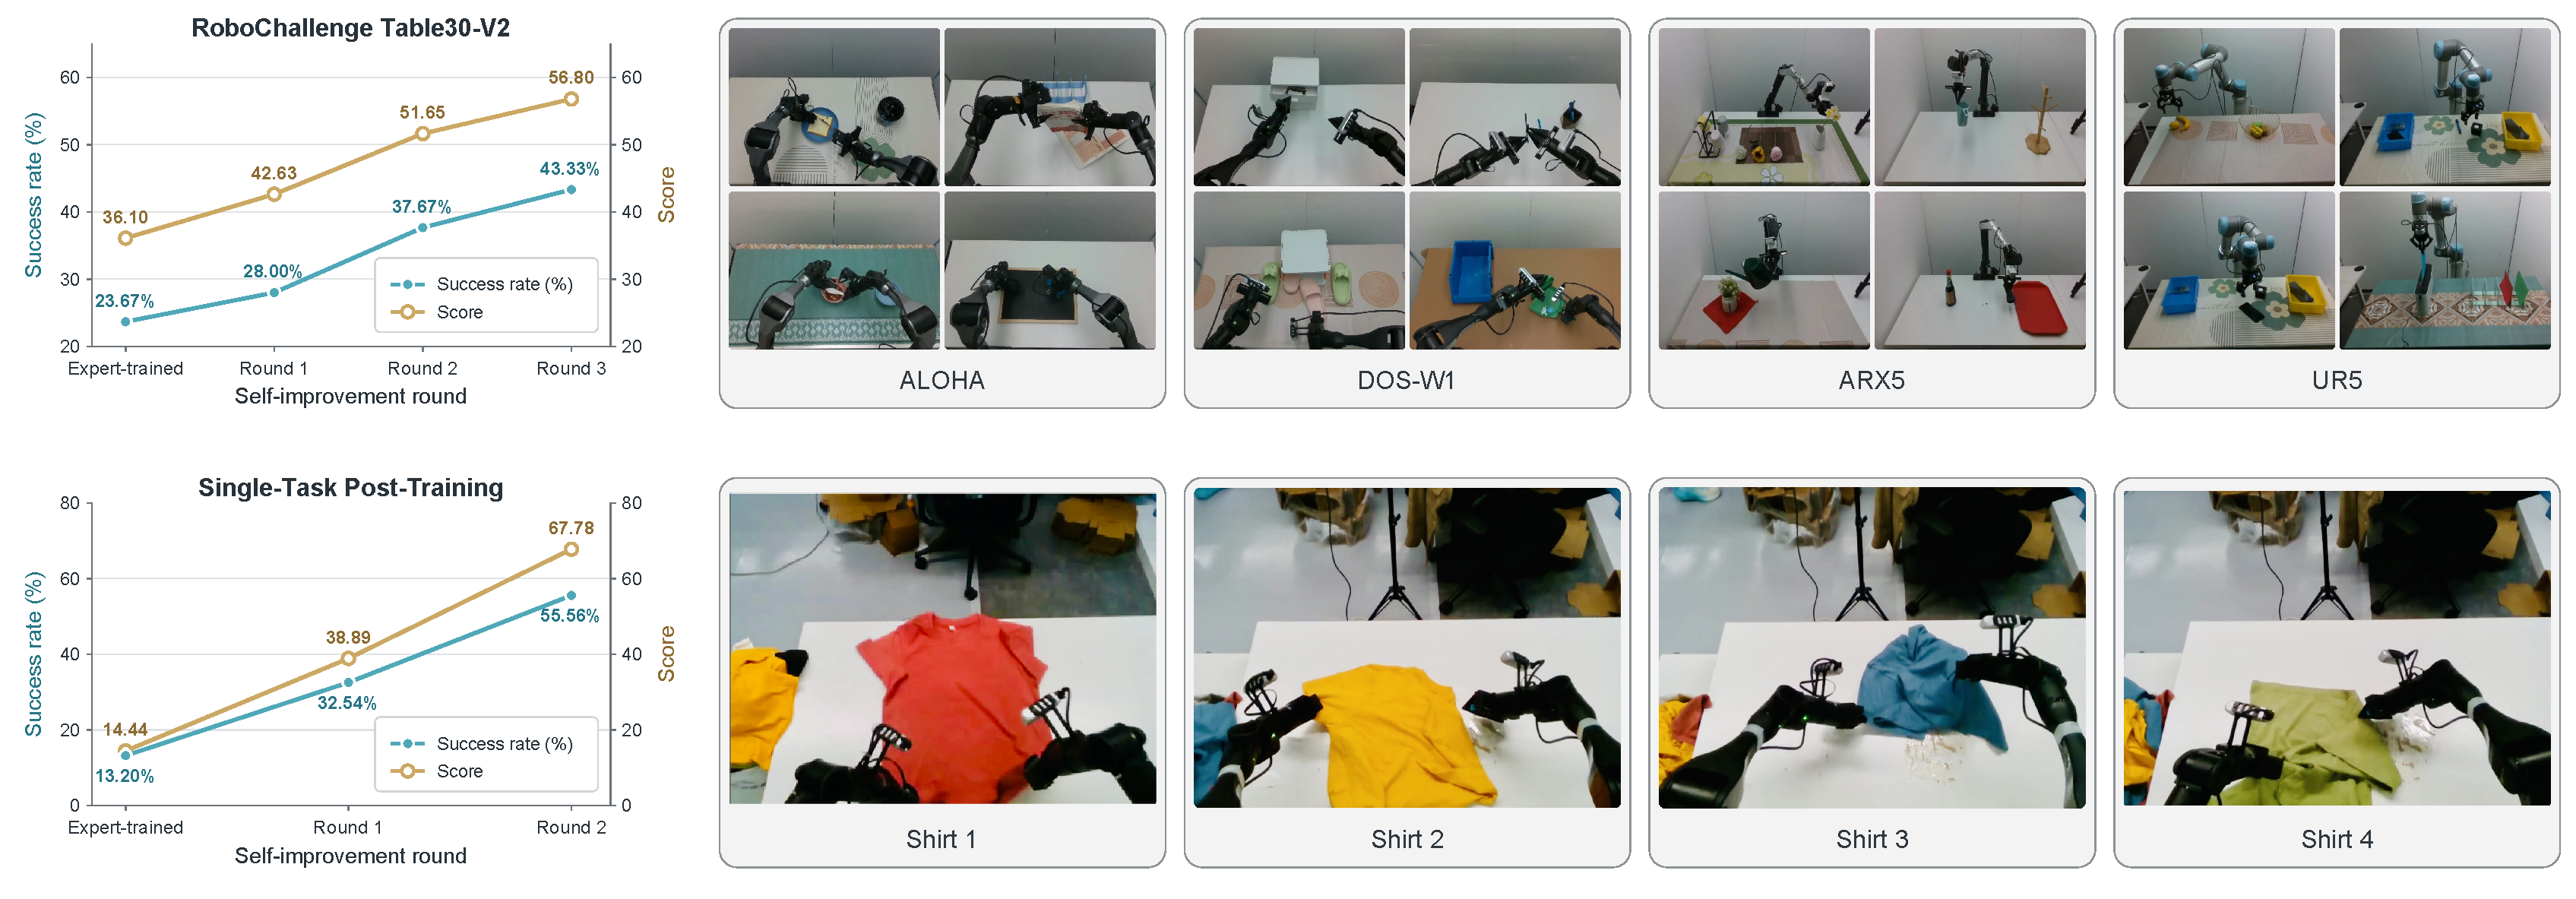
\includegraphics[width=\linewidth]{figures/closed_loop_improvement.pdf}
    \caption{Closed-loop improvement from real-robot deployment. 
    Top: three deployment-and-training iterations on RoboChallenge Table30-V2, covering 30 tasks across four robot embodiments. 
    Bottom: two deployment-and-training iterations on shirt folding after task-specific expert post-training of the DOS-W1 model. 
    Each plot reports success rate and score over successive improvement rounds.}
    \label{fig:closed_loop_improvement}
\end{figure}

We examine deployment-driven improvement in two real-robot settings: multi-task learning and single-task post-training (Figure~\ref{fig:closed_loop_improvement}).
Both follow the update procedure in Section~\ref{sec:deployment_loop}: At each iteration, we deploy the current policy and assign quality scores to the collected rollouts, then update the model through quality-aware joint training on expert demonstrations and all rollouts collected so far.

\textbf{Multi-task deployment.}
As in Section~\ref{sec:benchmark_setup}, we train multi-task models for ALOHA, DOS-W1, ARX5, and UR5, covering the 30 Table30-V2 tasks.
Starting from expert-trained checkpoints, each model undergoes three rounds of deployment and training using experience from its assigned tasks.
Overall success increases from 23.67\% to 28.00\%, 37.67\%, and 43.33\%, while the scores rise from 36.10 to 42.63, 51.65, and 56.80.
Both aggregate metrics improve at every iteration, yielding a 19.7-percentage-point success gain over the initial deployment.
This demonstrates that LoopWAM can use its own deployment experience to improve policies trained across multiple tasks.

\textbf{Single-task post-training.}
We further evaluate shirt folding, a challenging deformable-object manipulation task with diverse and disordered initial configurations.
A shirt is casually tossed into the robot's workspace, creating varied and messy initial states in which its corners may be hidden.
The robot must identify suitable grasp points and progressively unfold the shirt until its corners are exposed, then grasp these corners to complete the subsequent folds.
We initialize from the DOS-W1 multi-task model trained on Table30-V2 and post-train it on newly collected expert demonstrations of shirt folding.
The resulting task-specific expert-trained checkpoint serves as the starting point for two rounds of deployment and self-improvement.
Success rises from 13.20\% to 32.54\% and 55.56\%, while the scores increase from 14.44 to 38.89 and 67.78.
These gains show that deployment feedback remains effective after adapting a multi-task model to a challenging individual task, supporting closed-loop improvement under both training regimes.

\subsection{Ablation Study}
\label{sec:ablation}

We use the RoboTwin~2.0 setup in Section~\ref{sec:benchmark_setup}, varying only quality steering and rollout action supervision; expert action supervision and video supervision remain unchanged.

% !TEX root = ../main.tex
\begin{table*}[t]
\caption{Ablation study on RoboTwin~2.0. We evaluate quality steering with different annotation schemes and assess the effect of quality-weighted rollout action supervision (Act.).}
\label{tab:robotwin_ablation}
\centering
\small
\setlength{\tabcolsep}{4pt}
\renewcommand{\arraystretch}{1.0}
\setlength{\resulttablewidth}{0.75\linewidth}
\begin{tabular*}{\resulttablewidth}{l@{\extracolsep{\fill}}cccc}
    \toprule
    Quality Steering & Quality-weighted Act. & Clean & Rand. & Average \\
    \midrule
    None & \xmark & 73.5 & 71.1 & 72.3 \\
    Extra-coarse & \xmark & 92.2 & 93.3 & 92.8 \\
    \resultrow{secondsky}Extra-coarse & \cmark & 93.9 & 93.3 & 93.6 \\
    Coarse & \xmark & 93.2 & 92.2 & 92.7 \\
    \midrule
    \resultrow{loopsky}\textbf{Coarse (ours)} & \cmark & \textbf{94.6} & \textbf{94.4} & \textbf{94.5} \\
    \bottomrule
\end{tabular*}
\end{table*}


Table~\ref{tab:robotwin_ablation} compares no steering, extra-coarse annotation, and our coarse-level annotation (Section~\ref{sec:quality_steering}).
Extra-coarse annotation distinguishes rollouts from all policies solely by success or failure: all failed rollouts are assigned \textit{Quality: low}, all successful rollouts are assigned \textit{Quality: medium}, and expert demonstrations are assigned \textit{Quality: high}.
In our coarse-level scheme, successful rollouts from the same policy are assigned a shared numerical score, which can differ across policies according to their overall success rates across tasks and manually assessed motion smoothness.
Failed rollouts are assigned the minimum score, while expert demonstrations are assigned $q^\star$, above the rollout score range. The ablation results reveal three key findings: 
\textbf{(1)} Quality steering is key to learning from mixed-quality deployment rollouts, enabling the model to distinguish trajectories of different quality.
\textbf{(2)} Even extra-coarse labels remain effective, demonstrating that fine-grained annotation is not required to benefit from steering.
\textbf{(3)} Quality-aware rollout action supervision further improves overall performance under both annotation schemes.

